

%%%%%%%%%%%%%%%%%%%%% LateX template %%%%%%%%%%%%%%%%%


%%%%%%%%%%%% inicio del documento incluyendo opciones %%%%%%%%%%%%%%%%%%%%%%%%%%%%%%%
\documentclass[letterpaper,11pt]{article}
%%%%%%%%%%%%%%%%%%%%%%%%%%%%%%%%%%%%%%%%%%%%%%%%%%%%%%%%%%%%%%%%%%%%%%%%%%%%

%%%%%%% paquetes utiles: español, incluir graficos, etc %%%%%%%%%%%%%%%%%%%%%%%%%%%%
\usepackage[utf8]{inputenc}
\usepackage{amsmath}
\usepackage{amsfonts}
\usepackage{amssymb}
\usepackage{amsthm}
\usepackage[spanish]{babel}
\usepackage{latexsym}
\usepackage{euscript}
\usepackage{graphicx}
\usepackage{tdclock}
\usepackage{braket}
\usepackage[autostyle=true]{csquotes}
\usepackage{braket}
\usepackage{pdfpages}
\usepackage{subcaption}
\usepackage{hyperref}
%%%%%%%%%%%%%%%%%%%%%%%%%%%%%%%%%%%%%%%%%%%%%%%%%%%%%%%%%%%%%%%%%%%%%%%%%%%%%%%%%%

%%%%%%%%%%%%%%%%%%% espacio para la primera linea del parrafo %%%%%%%%%%%%%%%
\setlength{\parindent}{0mm} 
%%%%%%%%%%%%%%%%%%%%%%%%%%%%%%%%%%%%%%%%%%%%%%%%%%%%%%%%%%%%%%%%%%%%%%%%%%

%%%%%%%%%%%%%%% espacio entre parrafos %%%%%%%%%%%%%%%%%%%%%%%%%%%%%%%
\setlength{\parskip}{2mm}
%%%%%%%%%%%%%%%%%%%%%%%%%%%%%%%%%%%%%%%%%%%%%%%%%%%%%%%%%%%%%%%%%%%%

%%%%%%%%%%%%%%%%%%%%% espaciado entre lineas %%%%%%%%%%%%%%%%%%%%%%%%%%%%%
\linespread{1} 
%%%%%%%%%%%%%%%%%%%%%%%%%%%%%%%%%%%%%%%%%%%%%%%%%%%%%%%%%%%%%%%%%%%%%%

\renewcommand{\vec}[1]{\mathbf{#1}}

%%%%%%%%%%%%%%%%%%%%%%%% Control de margenes %%%%%%%%%%%%%%%%%%%%%%%%%%%%
%\setlength{\topmargin}{-1.cm}
\setlength{\oddsidemargin}{-.8cm}
\setlength{\evensidemargin}{-.8cm}
\setlength{\textheight}{24cm} 
\setlength{\textwidth}{18cm} 
\setlength{\headsep}{-2cm}
%%%%%%%%%%%%%%%%%%%%%%%%%%%%%%%%%%%%%%%%%%%%%%%%%%%%%%%%%%%%%%%%%%%%%%%%%%%%

%%%%%%%%%%%%%%%  definicion de comandos que se utilicen frecuentemente %%%%%%%%%%%%%%%
\def\und#1{\underline{#1}}
\def\be{\begin{equation}}
\def\ee{\end{equation}}
\def\bea{\begin{eqnarray}}
\def\eea{\end{eqnarray}}
%%%%%%%%%%%%%%%%%%%%%%%%%%%%%%%%%%%%%%%%%%%%%%%%%%%%%%%%%%%%%%%%%%%%%%%%%%%%%%%%%%%%

%%%%%%%%%%% Aqui se inicia el contenido del documento %%%%%%%%%%%%%%%%%%%%%%%%%%%%%%%%
\begin{document}

\begin{center}
{\bf \Large Doble péndulo} 
\end{center}

\noindent
{\bf \large Carlos Manuel Rodríguez Martínez} \hspace{5.2cm}

\smallskip
El \textit{doble péndulo} es un ejemplo de sistema mecánico que pone en evidencia la complejidad que pueden generar este tipo de sistemas de construcción simple. Este sistema en su forma más simple está formado por dos masas colgando de cuerdas de masa despreciable y sin fricción, donde las masas están sujetas a la acción de la gravedad (figura \ref{fig:penddoblediag}). Se desea describir el movimiento de ambas masas.

\begin{figure}[h!]
\centering
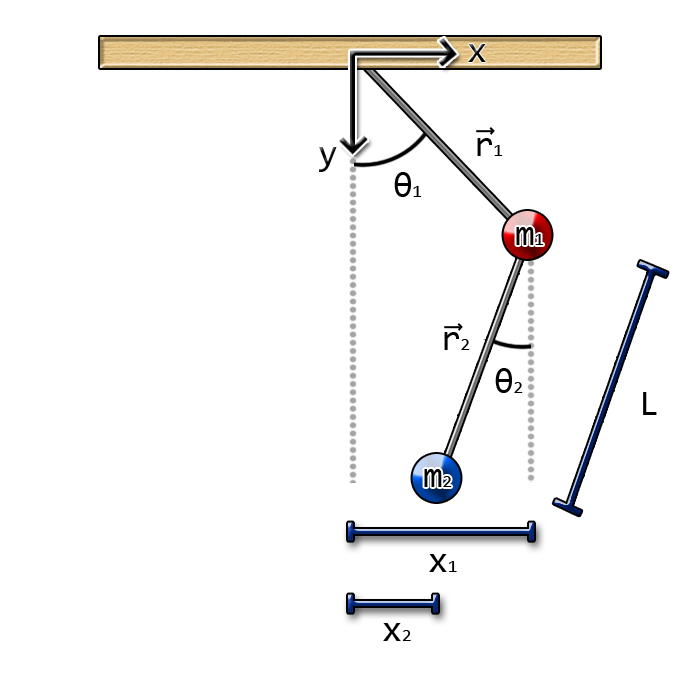
\includegraphics[scale=0.35]{img/PendDobleDiag}
\caption{Diagrama del péndulo doble.}
\label{fig:penddoblediag}
\end{figure}

Se define al vector $\vec{r_1}$ en función de los ángulos $\theta_1$ y $\theta_2$ como
\[
	\vec{r_1} = l \left(\hbox{sen}(\theta_1)\hat{i} + cos(\theta_1)\hat{j} \right) ,
\]
cuya derivada es
\[
	\dot{\vec{r_1}} = l\dot{\theta_1} \hbox{cos}(\theta_1)\hat{i}-l\dot{\theta_1} \hbox{sen}(\theta_1)\hat{j}.
\]
Entonces el cuadrado del módulo de $\dot{\vec{r_1}}$ es
\begin{equation}
	\dot{\vec{r_1}}^2 = l^2 \dot{\theta_1}^2.
\end{equation}
Análogamente para $\vec{r_2}$
\[
	\vec{r_2} = l \left( \hbox{sen}(\theta_1) + \hbox{sen}(\theta_2) \right) \hat{i} + l \left(\ hbox{cos}(\theta_1) + \hbox{cos}(\theta_2) \right) \hat{j}.
\]
Su derivada
\[
	\dot{\vec{r_2}} = \left((\dot{\theta_1}l \hbox{cos}(\theta_1) + \dot{\theta_2}l \hbox{cos}(\theta_2) \right) \hat{i} - \left(\dot{\theta_1}l \hbox{sen} (\theta_1) + \dot{\theta_2}l \hbox{sen} (\theta_2) \right) \hat{j}.
\]
El cuadrado de su módulo es
\begin{equation}
	\dot{\vec{r_2}} = l^2 \left[\dot{\theta_1}^2 + \dot{\theta_2}^2 + 2\dot{\theta_1}\dot{\theta_2} \hbox{cos}(\theta_1-\theta_2) \right],
\end{equation}
de esta manera se puede describir la energía cinética del sistema como
\begin{align}
	T &= T_1 + T_2 = \frac{1}{2} m_1 \dot{\vec{r_1}} + \frac{1}{2} m_2 \dot{\vec{r_2}} \nonumber \\
	 &= \frac{1}{2} m_1 l^2 \dot{\theta_1}^2 + \frac{1}{2} m_2 l^2 \left[\dot{\theta_1}^2 + \dot{\theta_2}^2 + 2\dot{\theta_1}\dot{\theta_2} \hbox{cos}(\theta_1-\theta_2) \right] \nonumber \\
	 &= \frac{1}{2} l^2 \left[\dot{\theta_1}^2 (m_1 + m_2) + \dot{\theta_2}^2 m_2 + 2 m_2 \dot{\theta_1} \dot{\theta_2} \right] \nonumber,
\end{align}
y la energía potencial se define como
\begin{align}
	V &= V_1 + V_2 = m_1 g r_{1y} + m_2 g r_{2y} = -m_1 g l \hbox{cos}(\theta_1) - m_2 g l( \hbox{cos}(\theta_1)+ \hbox{cos}(\theta_2)) \nonumber \\
	  &= -gl((m_1+m_2) \hbox{cos} (\theta_1)+m_2 \hbox{cos}(\theta_2)) \nonumber.
\end{align}
De estas magnitudes se obtiene el lagrangiano $L = T - V$,
\begin{align}
	L = \frac{1}{2} l^2 \left[\dot{\theta_1}^2 (m_1 + m_2) + \dot{\theta_2}^2 m_2 + 2 m_2 \dot{\theta_1} \dot{\theta_2} \right] \nonumber \\
				+ gl \left((m_1+m_2) \hbox{cos} (\theta_1)+m_2 \hbox{cos}(\theta_2) \right).
\end{align}
Utilizando la ecuación de Euler-Lagrange se obtienen las ecuaciones de movimiento para el sistema.
Despejando para $\theta_1$,
\begin{align}
	{d\over dt }\left[ \frac{1}{2} l^2 (2 \dot{\theta_1}(m_1 + m_2) + 2m_2 \dot{\theta_2} \hbox{cos} (\theta_1 - \theta_2)) \right] \nonumber \\
	= -gl(m_1 + m_2) \hbox{sen} (\theta_1) - m_2 \dot{\theta_1} \dot{\theta_2} l^2 \hbox{sen} (\theta_1 - \theta_2) \nonumber,
\end{align}

\begin{align} \label{eq:pend_th1}
	l^2 \ddot{\theta_1} (m_1 + m_2) + m_2 l^2 \ddot{\theta_2} \hbox{cos}(\theta_1 - \theta_2) = -m_2 l^2 \dot{\theta_2}^2 \hbox{sen} (\theta_1 - \theta_2) \nonumber \\
	- gl(m_1 + m_2) \hbox{sen} (\theta_1).
\end{align}
Despejando para $\theta_2$,
\begin{align}
	{d\over dt }\left[ \frac{1}{2} l^2 (2m_2 \dot{\theta_2} + 2m_2 \dot{\theta_1} \hbox{cos} (\theta_1 - \theta_2)) \right] \nonumber \\
	= -g l m_2 \hbox{sen}(\theta_2) + l^2 m_2 \dot{\theta_1} \dot{\theta_2} \hbox{sen} (\theta_1 - \theta_2) \nonumber,
\end{align}

\begin{align} \label{eq:pend_th2}
	l^2 m_2 \ddot{\theta_2} + l^2 m_2 \ddot{\theta_1} \hbox{cos} (\theta_1 - \theta_2) = m_2 l^2 \dot{\theta_1}^2 \hbox{sen}(\theta_1 - \theta_2) \nonumber \\
	- g l m_2 \hbox{sen}(\theta_2).
\end{align}
Aquí se tiene un sistema de dos ecuaciones (\ref{eq:pend_th1} y \ref{eq:pend_th2}) y dos incógnitas $\theta_1$ y $\theta_2$. De aquí se obtienen las ecuaciones de movimiento para este sistema:
\begin{equation}
	\ddot\theta_1 = \frac {-g (2m_1+m_2)\hbox{sen} \theta_1 -m_2g \hbox{sen}(\theta_1-2\theta_2)-
	2\hbox{sen}(\theta_1-\theta_2)m_2(\dot\theta_2^2 l_2 + \dot\theta_1^2 l_1\hbox{cos}(\theta_1-\theta_2))}
	{l_1(2m_1+m_2-m_2 \hbox{cos}(2\theta_1 -2\theta_2))}
\end{equation}
y 
\begin{equation}
	\ddot\theta_2 = \frac {2 \hbox{sen}(\theta_1 - \theta_2) (\dot\theta_1^2 l_1 (m_1 + m_2) 
	+ g(m_1 + m_2) \hbox{cos} \theta_1 + \dot\theta_2^2 l_2 m_2 \hbox{cos}(\theta_1 - \theta_2)) } 
	{l_2 (2 m_1 + m_2 - m_2 \hbox{cos}(2 \theta_1 - 2 \theta_2))}.
\end{equation}

No es posible obtener la solución en términos de funciones elementales para este par de ecuaciones diferenciales, lo que pone en evidencia la naturaleza caótica del sistema. A la hora de resolver este tipo de sistemas se suelen utilizar métodos numéricos como el método de Euler o Runge-Kutta.

\begin{figure}[h!]
\centering
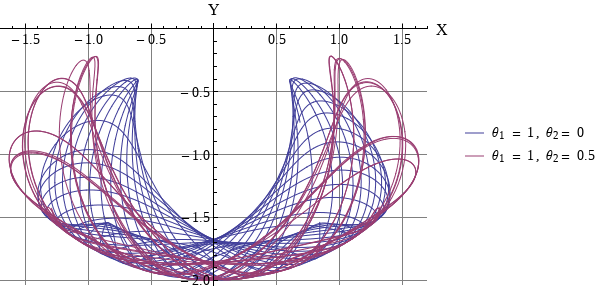
\includegraphics[scale=0.60]{img/PendDobleTray}
\caption{Trayectoria del péndulo doble.}
\label{fig:penddobletray}
\end{figure}

En la figura \ref{fig:penddobletray} se puede ver la dinámica caótica de la trayectoria del segundo péndulo variando ligeramente las condiciones iniciales. Este ejemplo sirve para ilustrar la naturaleza caótica de un sistema simple en apariencia y, por lo mismo, para resolverlo es necesario hacer uso de una simulación por métodos numéricos.


\end{document}

